\documentclass[11pt]{article}
\usepackage[subpreambles=true]{standalone}

\usepackage{acl2012}
%\usepackage{times}
\usepackage{latexsym}
%\usepackage{fontspec}
%\usepackage[final]{microtype}
%\usepackage{flushend}


\usepackage[author={Lyndon White}]{pdfcomment}

\usepackage[boxed]{algorithm2e}


\usepackage{verbatim}
\usepackage{grffile}
%\usepackage[draft]{graphicx}

\usepackage{pgfplots}
\pgfplotsset{compat=1.12}
\usepackage{booktabs, array} % Generates table from .csv
\usepackage{pgfplotstable}

\usepackage{tikz}
\usetikzlibrary{positioning}
\usepackage{xifthen}

%%%%%%%%%%MATH
\usepackage{amsthm}
\usepackage{amsmath}
\usepackage{amssymb}
\usepackage{amsfonts}

\theoremstyle{plain}
\newtheorem{thm}{\protect\theoremname}
\theoremstyle{definition}
\newtheorem{defn}[thm]{\protect\definitionname}
\usepackage{csquotes}
\usepackage[english]{babel}
\providecommand{\definitionname}{Definition}
\providecommand{\theoremname}{Theorem}
%%%%%



%\hypersetup{draft} %Avoid hyperef causing issuse when links broken over pages by disabling hyperref

\usepackage[backend=bibtex,
 style=authoryear-icomp,
 bibencoding=ascii,
 maxcitenames=2,
 url=false,
 hyperref=false
]{biblatex}
\bibliography{master}

\usepackage{cleveref}


%End Packages

%%%%%%%%%%%%%%%%%%%%%% Magic Float Layer Fix Settings 
\renewcommand{\topfraction}{.85}
\renewcommand{\bottomfraction}{.7}
\renewcommand{\textfraction}{.15}
\renewcommand{\floatpagefraction}{.66}
\renewcommand{\dbltopfraction}{.66}
\renewcommand{\dblfloatpagefraction}{.66}
\setcounter{topnumber}{9}
\setcounter{bottomnumber}{9}
\setcounter{totalnumber}{20}
\setcounter{dbltopnumber}{9}

%%%%%%%%%%%%%%%%%



\DeclareMathOperator*{\argmin}{argmin}

%%%%%%% Tables
\newcolumntype{C}[1]{>{\centering\arraybackslash}m{#1}}
\pgfplotstableset{
	columns/Model/.style={
		string replace={glove50}{50d GLoVE},
		string replace={glove100}{100d GLoVE},
		string replace={glove200}{200d GLoVE},
		string replace={glove300}{300d GLoVE},
		string type,
		column type=C{5.5em}		
	}	
} 

\pgfplotstableset{percent style/.style=}
		}},
		%
		%
		every head row/.style={after row=\midrule},
	}

%%%%%%



%opening
\title{Generating Sentences from the Sums of their Embeddings using a Greedy Algorithm}
\author{}
\graphicspath{{./figs/}}
\setlength\itemsep{2mm}
\begin{document}

\maketitle

\begin{abstract}
Converting a sentence to a meaningful vector representation has uses in many NLP tasks, however very few methods allow that representation to be restored to a human readable sentence. Being able to generate sentences from the vector representations is expected to open up many new applications. We introduce such a method for moving from sum of word embedding representations back to the original sentences. This is done using a greedy algorithm to convert the vector to a bag of words. We then show how the bag of words can be ordered using simple probabilistic language models to get back the sentence. To our knowledge this is the first work to demonstrate qualitatively the ability to reproduce text from a large corpus based on its sentence embeddings. 
As well as practical applications for sentence generation, the success of this method has theoretical implications on the degree of information maintained by the sum of embeddings representation.
\end{abstract}

\section{Introduction} \label{intro}
The task being tackled here is the \emph{resynthesis} of sentences from vector embeddings. In particular the generation of sentences from vectors based on the sum of their constituent words' embeddings. The generation task, going from vector to sentence, is quite challenging. It has not received a lot of attention.

The motivations for this work remain the same as in the first work in the area: \textcite{Dinu2014CompositionalGeneration}. From a theoretical perspective given that a sentence encodes its meaning, and the vector encodes the same meaning, then it must be possible to translate in both directions between the natural language and the vector representation. An implementation, such as the work reported in this paper, which demonstrates the truth of this dual space theory has its own value. There are also many potential practical applications of such an implementation, often ranging around certain types of ``translation'' tasks.

Given suitable bidirectional methods for converting between sentence vectors and sentences, the sentence vector space can be employed as a \emph{lingua franca} for translation between various forms of information. The most obvious of which is literal translation between different natural languages; however the use extends beyond this.

Several approaches have been developed for representing images and sentences in a common vector space. This is used to select a suitable caption a list of candidates \parencite{farhadi2010every,socherDTRNN}. The caption could instead be generated from the common vector space, through sentence resynthesis -- without any need for a list. There has also been significant recent work on this caption generation task directly using language generation, without the common space step, such as in \textcite{donahue2014long,Mao2014GenerateImageDesc}. The translation though common space approach suggested may provide a competing or supplementary technique for this task.

Another similar use is the replacement of vector based extractive summarisation \textcite{KaagebExtractiveSummaristation,yogatamaextractive}, with abstractive summarisation. The promising use of sentence generation for all these applications is to have a separate model trained to take the source information (e.g. a picture for image description, or a cluster of sentences for abstract summarisation) as its input and train it to output a sentence vector which can then be used to generate the sentence.

There are currently three existing methods for regeneration -- each tied to different machine learnt embedding representation. 
The current state of the art for full sentence generation are the works of \cite{iyyer2014generating} and \cite{Bowman2015SmoothGeneration}. 
Both these advance beyond the original work in the area of \cite{Dinu2014CompositionalGeneration} which is only theorised to extend beyond short phrases, both produce full sentences. These sentences are qualitatively shown to be loosely similar in meaning to the original sentences. Neither works has produced quantitative evaluation, making it hard to determine between them. Both are detailed further in the next.


The method proposed in this paper takes in a sum of word embeddings (SOWE) sentence vector, and outputs the sentence which it corresponds to. The input is a vector for example $\tilde{s}=[0.11, 0.57,-0.21,...,1.29]$, which approximates a SOWE vector, and outputs a sentence: for example "The boy was happy.". That input vector could come direct as the SOWE representation of a reference sentence (as is the case for the evaluation of our method presented in this paper). More practically it could come as the output of some other process; for example a machine learnt mapping from an image to the vector representation of its textual description. This vector representation is transformed through our process into a human readable sentence.

We extend the work of \textcite{White2015BOWgen}, which uses a greedy algorithm to generate bags of words (BOW), to generating sentences. This is done performing adding a word ordering step, after their selection step, as shown in \Cref{block_diagram}. The vector selection step is used to determine which words are in the sentence -- this converts the SOWE embedding into a bag of words. The new second step we propose is to order that bag of words into a sentence using a language modelling task. The second step is based on a variation of the Traveling Salesman based approach of \cite{Horvat2014}, implemented as a mixed integer programming (MIP) optimisation problem. The overall two step approach can generate proper sentences from SOWE vectors.
\begin{figure}
	\centering 
	\documentclass{standalone}

\usepackage{tikz}
\usetikzlibrary{positioning}


\begin{document}

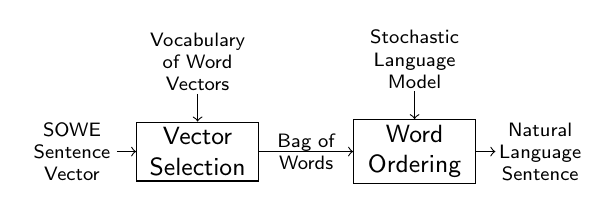
\begin{tikzpicture}[
	every node/.style={ text width=4em,
    					align=center,
                        font=\scriptsize\sffamily,
                        inner sep=1pt
                        },
	proc/.style= {draw,
    			  font=\small\sffamily,
                  inner sep = 2pt
    }
]
	\node (input) [inner sep=-4pt] {SOWE Sentence Vector};
    \node (selection) [proc, right = 0.7em of input]{Vector\\ Selection};
    \node (ordering) [proc, right = 3.4em of selection]{Word\\ Ordering};
	\node (vocab) [above = 1em of selection]{Vocabulary of Word Vectors};
    \node (lm) [above = 1em of ordering] {Stochastic Language Model};
    \node (output) [inner sep=-4pt, right=0.7em of ordering] {Natural Language Sentence};
    \draw[->] (input) -- (selection);
    \draw[->] (vocab) -- (selection);
    \draw[->] (selection) -- (ordering) node[midway] {Bag of Words};
    \draw[->] (lm) -- (ordering);
    \draw[->] (ordering) -- (output);
\end{tikzpicture}

\end{document}
	\caption{The process for the regenerating sentences from SOWE-type sentence vectors. \pdfcomment{Update diagram to refer to the input as the target vector}}
	\label{block_diagram}
\end{figure}

The rest of the paper is organized into the following sections. \Cref{relwork} introduces the area, discussing in general sentence models, and prior work on generation. \Cref{framework} explains the problem in detail and our algorithm for solving it. \Cref{evalsettings} described the settings used for evaluation. \Cref{results} presents the results on this evaluation. The paper concluded with \Cref{conclusion} and a discussion of future work on this problem.


\section{Related Works}\label{relwork}
\subsection{Embedding Models}

The compositional models come from classical linguistics -- based on the hierarchical  break-down of a sentence into clauses, phrases and words. Compositional vector models produce vectors by moving up the hierarchical tree combining (or ``composing'') the vectors for elements within a substructure to find the substructure's vector. This composition continues until the a vector has been found for the root of the sentence tree. The original work in this area is \textcite{Mitchell2008}. A variety of recursive neural network based methods were developed during the thesis of \textcite{socher2014recursive}. Compositional methods continue to improve, with newer methods as in \textcite{TACL15CompVector}, focusing on capturing with more efficiency and precision how words interact to control the meaning of their superstructures. 

%\textcite{socher2010PhraseEmbedding}%,SocherEtAl2011:RAE,SocherEtAl2011:PoolRAE,Socher2011ParsingPhrases,SocherMVRNN,RvNTN,SocherEtAl2013:CVG,Socher2013TensorReasoning}. Compositional embedding models have strong basis from their linguistic underpinnings.

Non-compositional embeddings allowing each word to more directly affect the overall sentence vector, rather than doing so through intermediate substructure vectors. This is a broad category covering all other embedding techniques. From the classic bag of words (BOW), and the simple sum of word embeddings (SOWE); to more complex approaches augmenting windowed language modelling neural networks with an addition sentence memory \parencite{le2014distributed}.  Non-compositional methods draw significant criticism for disregarding structure; BOW and SOWE draw additional criticism for entirely disregarding word order. However these weaknesses, while valid, may be offset by the improved discrimination allowed through words directly affecting the sentence vector -- without the potential lose in the repeated composing steps. This allows some non-compositional methods to be comparable overall to the more linguistically consistent compositional embeddings. 


Recently \textcite{White2015SentVecMeaning} found that when classifying real-world sentences into groups of semantically equivalent paraphrases, that using SOWE as the input resulted in very accurate classifications. In that work White et. al. partitioned the sentences into groups of paraphrases, then evaluated how well a linear SVM could classify unseen sentences into the class given by its meaning. They tested this using a variety of different sentence embeddings techniques as input to the classifier. They found that the classification accuracy when using SOWE as the input very similar to that of the best performing methods -- less that 0.6\% worse on the harder task. From this they concluded that the mapping from the space of sentence meaning to the vector space of the SOWE, resulted in sentences with the same meaning going to distinct areas of the vector space.

\textcite{RitterPosition} presents a similar task on spacial-positional meaning, which used carefully constructed artificial data, for which the meanings of the words interacted non-simply -- thus favouring the compositional models. In their evaluation the task was classification with a Naive Bayes classifier into one of five categories of different spatial relationships. Here also SOWE was found performing comparably and again even out performing the compositional models. The best of the SOWE models they evaluated, outperformed the next best model (compositional or otherwise) by over 5\%. These results suggest this simple method is still worth consideration. SOWE is the basis of the work presented in this paper.

\subsection{Sentence Generation from Vector Embeddings}

To our knowledge only three prior works exist in the area of sentence generation from vectors. The first two of which are based on compositional embeddings, while the most recent work at the time of this writing, is based on a non-compositional approach.

\newcommand{\p}{\tilde{p}_{1,2}}
\renewcommand{\u}{\tilde{u}}


\textcite{Dinu2014CompositionalGeneration}  extends the models described by \textcite{zanzotto2010estimating, Guevara2010} for generation. The composition is described as the sum of pair of linear transformations of the input vectors ($\u_1$ and $\u_2$) to get a output vector $\p$. Dinu and Baroni, investigate two sources for the input and target output vectors: word and short-phrase embeddings generated using the continuous bag of words method of \cite{mikolov2013efficient}, and the method used by \textcite{Guevara2010} using single value decomposition on the word and phrase co-occurrence matrix for the training data. The composition function is given by:  $$f_{comp}\::\:\mathbb{R}^d\times\mathbb{R}^d \to \mathbb{R}^d\::\: (\u_1, \u_2)\mapsto W_1\u_2+W_2\u_2$$
Likewise, decomposition can be described by: $$f_{decomp}\::\:\mathbb{R}^d\to \mathbb{R}^d\times\mathbb{R}^d \::\: \p \mapsto (W^\prime_1\p, W^\prime_2\p)$$.
During training linear transformation matrices $W_1$,$W_2$ and $W_1^\prime$,$W_2^\prime$ can be solved for using least squares regression.
While it theoretically generalises to whole sentences, by recursive application of the composition or decomposition functions, Dinu and Baroni's work is quantitatively assessed only on direct reconstruction only for decomposing Preposition-Noun and Adjective-Noun 2 word phrases. In the case where the  where the decomposition function was trained on vectors generated using the compositional function they were able to get perfect reconstruction on the word embedding based inputs.
% -- though as they note, this is not extremely difficult as it is fitting linear transformation to invert a linear transformation.

\renewcommand{\p}{\tilde{p}}

The work of \textcite{iyyer2014generating} is based on an extension of the unfolding recursive autoencoder \textcite{SocherEtAl2011:PoolRAE}. Recursive neural networks are jointly trained for both composing the sentence's words into a vector, and for decomposing that vector into words. This composition and decomposition is done by reusing a composition neural network at each vertex the  dependency tree structure with different weight matrices for each dependency relation. The total network is trained based on its accuracy to reproduce its input word vectors, through back-propagation. Through just using the top decomposing half of the network, from the sentence embedding up, it can be used to regenerate the words. This method was demonstrated quantitatively on five examples, shown in \Cref{results}; they show the generated sentences of \textcite{iyyer2014generating} to be loosely semantically similar to the originals.

%$$g_{comp}\:: (u_i)^N_{i=1} \mapsto \sigma(\sum_{i=1}^N W_i\u_i+\tilde{b})$$
%$$g_{decomp} \p \mapsto  (\sigma(W^\prime_i\p+\tilde{b}^\prime+W_{sib}\u^\prime_j)^N_{i=1}$$
%$\u^\prime_j$ is $g_{decomp}(p)_j$ if $j$ is the left most sibling of $i$ with the same dependancy relation to the parent as $i$ if one exists, or the zero vector otherwith
%Here $W_i$ and $W^\prime_i$ vary not by order, but by the dependency tree part of speech of the $i$th element.
%$\tilde{b}$ and $\tilde{b}^\prime$ are the biases.
%$\sigma$ is a nonlinear activation function, such as the sigmoid or the hyperbolic tangent functions. It is this nonlinearity that prevents the values being solved by any kind of least squares.

%Theoretically, even without the extensions the unfolding recursive auto-encoder could be used in the same way to generate sentences, however this has not been shown.


\textcite{Bowman2015SmoothGeneration} is an adaptation on the recurrent neural network language model of \textcite{mikolov2011RnnLM}, to produces and utilise a new type of non-compositional sentence embedding. Bowman et. al. devised a modification of the variational autoencoder  \parencite{kingma2013auto} with natural language inputs and outputs, to learn the sentence representations. These input and output stages are performed using long short-term memory recurrent neural networks \parencite{hochreiter1997long}. They demonstrate a number of uses of this technique, only one of which is sentence generation, in the sense of this paper.
While it is a generative model it does not seek to recreate a sentence purely from its vector input, but rather to produce a series of probability distributions on the words in the sentence. These distributions can be evaluated greedily, which the authors used to give three quantitative examples resynthesis (also shown in \Cref{results}). They found the sentence embeddings created were storing largely syntactic and loose topical information. 


Both \textcite{Dinu2014CompositionalGeneration}, and  \textcite{iyyer2014generating}, require an output structure to be provided for the decomposition. Like the method of  \textcite{Bowman2015SmoothGeneration}, the new method proposed in this paper does not require this structural information.

None of the existing methods have demonstrated recreation of the full sentence input close enough to allow for quantitative evaluation on a full corpus. They tend to output lose paraphrases, or roughly similar sentences -- itself a slightly distinct and useful task.  That is not the case for our method described in the next section, which can often exactly recreate the original sentence from its vector representation.


\subsection{Vector Selection}
\renewcommand{\c}{\tilde{c}}
\newcommand{\s}{\tilde{s}}
\newcommand{\x}{\tilde{x}}
\renewcommand{\t}{\tilde{t}}
\newcommand{\N}{\mathbb{N}}
\newcommand{\R}{\mathbb{R}}
\newcommand{\V}{\mathcal{V}}
\newcommand{\B}{\mathcal{B}}

Unlike current sentence generator models, the BOW generation method of \textcite{White2015BOWgen} generally outputs a BOW very close to the reference for that sentence -- albeit at the cost of loosing all word order information. It is because of this accuracy that we base our method upon it. We improve it for sentence generator by composing with a word ordering step. Without the word ordering them Vector Selection step we used is directly based on the greedy BOW generation method.

\textcite{White2015BOWgen} solves the BOW generation problem, by solving what they call the vector selection problem -- selecting the vectors that sum up closest to a given vectors. They formally define the vector selection problem is formally defined as:
\[
(\s,\V,\,d) \mapsto \argmin_{\left\{ \forall\c\in\N_{0}^{V}\right\} }\:d( \s,\,\sum_{\x_j\in\V}\:\x_{j}c_{j})
\]
to find the bag of vectors selected from the vocabulary set $\V$ which when summed is closest to the target vector $\s$. Closeness is assessed with distance metric $d$. $\c$ is the indicator function for that multi-set of vectors. As there is a one to one correspondence between word embeddings and their words, finding the vectors results in finding the words. \textcite{White2015BOWgen} propose a greedy solution to the problem.
 
The principle part of algorithm of \textcite{White2015BOWgen} is greedy addition. Using this process they greedy add vectors to a partial solution building towards a complete bag. They start with a empty bag of word embeddings, and at each step add the vector which when added to the current partial solution, results in minimal distance to the target -- when compared to other vectors from the vocabulary. They continue repeating this step, until there is no vectors in the vocabulary that can be added without moving away from the solution. Then they use a fine-tuning method called n-substitution to avoid some greedy mistakes.

The n-substitution method avoids mistakes by examining partial solutions (bags of vectors) and seeing if it is possible to find a better solution by removing n elements and replacing them with up-to n different elements. The replacement search is exhaustive over the n-ary cartesian product of the vocabulary. Only for $n=1$ is it current feasible for practical implementation outside of highly restricted vocabularies. Never-the-less even 1-substitution can be seen as lessening the greed of the algorithm, though allowing early decisions (of which vectors to being include) to be reconsidered in the full context of the partial solution. The algorithm does remain greedy, but many simple mistakes are avoided by n-substitution. \textcite{White2015BOWgen} repeat greedy addition and n-substitution until the solution converges.




\section{General Framework}\label{framework}
As discussed in \Cref{intro}, and shown in \Cref{block_diagram}, the approach taken to generate the sentences from the vectors comes in two steps. First selecting the words used -- this is done deterministically, based on a search of the embedding space. Followed by ordering them, here demonstrated using a classic stochastic language modelling approach. The separating of the process into two steps is unlike any of the existing methods for sentence generation from vectors. The two subproblems which result from this split resemble more classical computer science problems. The selection problem, of choosing the best word vectors to sum to the target is a knapsack-like problem. The word-ordering problem is a search for the most-likely path through a Markov graph of n-gram probabilities. It may be noted, that both these sub-problems are NP-hard.


\subsection{The Ordering Problem} \label{ordering}
\begin{figure*}
	\documentclass{standalone}
\usepackage{arrayjobx}
\usepackage{xifthen}
\usepackage{tikz,textcomp}
\usepackage{ amssymb }

\begin{document}
	
\tikzset{ shorten <>/.style={ shorten >=0.2cm, shorten <=0.2cm } }

\begin{tikzpicture}
\newarray\Words
\readarray{Words}{$w_\triangleright$&$w_1$&$w_2$&$w_3$&$w_4$&$w_\triangleleft$}
\dataheight=5

\newcommand{\ystep}{0.5}

\newcommand{\gx}{}
\newcommand{\gy}{}


\newcommand{\drawgroupinner}{
	\foreach \j in {1,...,6}
	{
		\colorlet{MyColor}{black}%
		\ifthenelse{\i=\j}{\colorlet{MyColor}{gray}}{}
		\ifthenelse{\j=1}{\colorlet{MyColor}{gray}}{}
		
		\node[MyColor] (w_\i\j) at (\gx,\gy-\ystep*\j cm) {\Words(\i)\Words(\j)};
	}
	\draw (\gx,\gy-3.5*\ystep cm) ellipse (0.7cm and \ystep*4 cm);
}

\newcommand{\drawgrouptop}[3]{%
	\renewcommand{\i}{#1}
	\renewcommand{\gx}{#2 cm}
	\renewcommand{\gy}{#3 cm}
	\drawgroupinner{}	
	\node at (\gx,\gy+1*\ystep cm) {$S($\Words(\i)$)$};

}
\newcommand{\drawgroupbottom}[3]{%
	\renewcommand{\i}{#1}
	\renewcommand{\gx}{#2 cm}
	\renewcommand{\gy}{#3 cm}
	\drawgroupinner{}	
	\node at (\gx,\gy-8*\ystep cm) {$S($\Words(\i)$)$};	
}



\drawgrouptop{1}{0}{0}
\drawgrouptop{2}{2.5}{2.5}
\drawgroupbottom{3}{5}{-1.5}
\drawgrouptop{4}{7.5}{2.5}
\drawgrouptop{5}{10}{0}



\foreach \i in {1,...,5}
{	
	\foreach \j in {2,...,5}
	{
		\colorlet{MyColor}{black}%
		\ifthenelse{\j=2}{\colorlet{MyColor}{cyan!50!black}}
		{\ifthenelse{\j=3}{\colorlet{MyColor}{blue!50!black}}%
%		{\ifthenelse{\j=3}{\colorlet{MyColor}{red!50!black}}%
		{\ifthenelse{\j=4}{\colorlet{MyColor}{yellow!50!black}}%
		{\ifthenelse{\j=5}{\colorlet{MyColor}{green!50!black}}%
		{}}}}%}


		\ifthenelse{ \NOT \i=\j}{
			\foreach \k in {2,...,6}
			{
				\ifthenelse{\NOT \k=\i \AND \NOT \k=\j}
				{
					\draw[->,MyColor] (w_\i\j) -- (w_\j\k);
				}{}
			}
		}{}
	}
}

\node (w_S) at (-2cm,-1.5) {$w_\blacktriangleright$\Words(1)};
\draw (-2cm,-1.5) ellipse (0.7cm and 1 cm);
\node at (-2cm,-1.5cm +1.3 cm) {$S(w_\blacktriangleright)$};


\foreach \j in {2,...,5}
{
	\draw[->, red!70!black] (w_S)  --  (w_1\j);
}


\node (w_E) at (12cm,-1.5) {\Words(6)$w_\blacktriangleleft$};
\draw (12cm,-1.5) ellipse (0.7cm and 1 cm);
\node at (12cm,-1.5cm +1.3 cm) {$S($\Words(6)$)$};
\foreach \j in {1,...,5}
{
	\draw[->, red!70!black] (w_\j6) -- (w_E);
}

%\draw[->,line width=1mm,brown] (w_S) -- (w_12) -- (w_23)--(w_34)--(w_45)--(w_56)--(w_E);

\end{tikzpicture}

\end{document}
	\caption{\label{fig:ordergraph} A graph showing the legal transitions between states, when the word-ordering problem is expressed similar to a GA-TSP. Each edge $(w_aw_b)\to (w_bw_c)$ has cost $-\log(P(w_c\:|\:w_aw_b)$}. The nodes are grouped into columns for each district (word). In bold is shown one legal path which goes from beginning, to end, and covers all districts (words). 
\end{figure*}

After the bag of words has been generated by the previous step, it must be ordered. For example “are how , today hello ? you”, is to be ordered into the sentence: “hello , how are you today ?”. This problem can not always be solved to a single correct solution. \textcite{Mitchell2008}  gives the example of "It was not the sales manager who hit the bottle that day, but the office worker with the serious drinking problem." which has the same word content (though not punctuation) as "That day the office manager, who was drinking, hit the problem sales worker with a bottle, but it was not serious.". However, while a unique ordering can not be guaranteed, finding the most likely word ordering is possible.

Our method for word ordering is to formulate the problem as a linear mixed order programming problem (MIP). This lets us take advantage of the efficient existing solvers for this problem. Extending the work of \textcite{Horvat2014} we expressed the problem in a variation of a generalised asymmetrical travelling salesman problem (GA-TSP) -- which we then express as a MIP. 

The word-ordering problem is expressed as a GA-TSP, by mapping trigram states, to nodes, transition probabilities to edge costs, and words to districts. A diagram for the ordering of a BOW of size five is shown in \Cref{fig:ordergraph}.

The constraint on out problem variation are largely similar to a GA-TSP. 

The each word in the BOW is ascribed an arbitrary index. For words occurring with multiplicity greater than 1, they are ascribed a multiple indices, and treated as per differing words. The sentences are supplemented with pseudowords, with two placed a the beginning (represented by $w_\triangleright$ and $w_\blacktriangleright$)) and end (represented by ($w_\triangleleft$ and $w_\blacktriangleleft$)) of the sentences. These pseudowords allow the trigram language model to indicate information about the words which occur near the sentence boundaries.

Each node corresponds to a pair of words, corresponding to the previous two words before the edge. This is the markov state for the trigram language model. Each edge is a transition between these states and has cost given by the language model. $w_aw_b\to w_bw_c$ has cost given by $-\log(P(w_c\:|\:w_aw_b)$. Only no transition of $w_aw_b\to w_cw_d$ for $b\ne c$ are allowed. This is one of several constraints on the problem.

The key constraint on the path is that every node entered, must be exited. For example as if there is the transition $w_1w_2 \to w_2w_3$ then having a transition $w_2w_4\to w_4w_5$ would not be allowed, as that would have a "jump" within the district  of $w_2$ -- which is not a continuous path. The exception to this is the end node ($w_\triangleleft w_\blacktriangleleft$), which does not have to be exited.

As in normal in a GA-TSP, there is the requirement that every district is visited once. In this case the districts correspond to having a word in the state. Every word ($w_i$), must be used once. In \Cref{fig:ordergraph} the districts are based on the first index of the state. Similar equivalent rules can be defined from the second index.
 
Beyond this, we went on to express the problem further into a MIP form. This meant the use with a a MIP solver, rather than a TSP solver. This direct expression allowed us to vary the problem, with the potential for small optimisations.



Normally, for a problem with known start and end vertices to be considered as a travelling salesman problem, the vertices are connected with a zero cost link. As there are exactly one Start and End pseudo-word states we simply special case them in the MIP definition as not requiring incoming or outgoing connections, respectively. We also made direct use of the knowledge that the Start and End states must to always occur in every tour, to simplify the sub-tour elimination. 

When the travelling salesman problem is solved as a MIP,  some potential solutions contain non-connected subtours. These are eliminated by adding new "lazy" constraints are added, each time such a solution is suggested. For the normal TSP, subtours are eliminated with the constraint that every subtour must have an additional outgoing connection to one of the other subtours. This is more complex in case of the generalised asymmetrical TSP: for each subtour there must an outgoing connection from the nodes of the neighbours covered by it, to one of the nodes in the union of the neighbourhoods covered by the other subtours. Finding these unions takes a non-negligible amount of time; but only one of them is needed to eliminate this subtour. When multiple subtours are common adding multiple constraints cause more to be eliminated; however we've found that subtours are rare in the word ordering problems, and multiple subtours even more so -- as such, pre-emptively adding constraints to eliminate them is not efficient computationally. We can quickly find the core tour, by following the path from the Start to the End pseudo-word states. Then we add only the requirement that there is an outgoing connection from the nodes in neighbourhoods covered by the core tour, to one or more of the nodes outside that set. Preliminary testing found this to give a marginal speed-up.

In going forward, expressing the problem directly as a MIP rather than a GA-TSP opens several avenues. It is simple to get the second, third and so forth best solution, by adding a standard MIPs constraint to disallow the better solutions. It also is open to relaxation of constraints. 

When the constraints on the MIP problem render no solution feasible, this prevent an solution being found. For example, there is no possible ordering of most BOW that do not contain a period, question mark, or exclamation mark. Adjustments can be made to the MIPs model to detect this being that cause of the infeasibility (using irreducible inconsistent subsystem methods), this would then allow for suitable relaxations to the constraints to be applied to generate solutions to the problem.



\begin{comment}
We first formulate the problem into a Markov graph of states (each correspond to potential subsequences of two words), with edges weighted according to the log of the trigram possibility of the transitions between them 

The probability of any sequence of words can be found using a trigram language model. We can express all possible orderings as a graph between Markov states of the last two words, connected to allowable following words by edged weighted by the negative log of the trigram probability. 
 with edges weighted with the logThis language model can be used to 


The problem for ordering is assign an map between 

The problem can be expressed in terms of a Markov  chain
In this section a demonstration of the feasibly of solving for the correct word order, given the output of the previous step is shown. This is a stochastic language modelling problem -- to determine the most likely sequence of words, given the constraints that the words are exactly those given by the BOW output from the previous step. The method presented here is simply to show its feasibility; the development of efficient technique for use in the ordering problem is left for future work.\pdfcomment{LW: I think this sentence/paragraph can be cut down a lot. RT: I agree, If this is a standard approach (used in ASR?) is there a need to describe the background of the beam seach using tri-gram models. YOu should just state what you implemented (with reference of where the beam search using trigrams is used), provide the parameter details in Section 4 and perhaps move the computational analysis (of all compoenents) into a separate section.}

For purposes of this demonstration a simple Kneser-Ney smoothed trigram model \parencite{kneser1995improved} was used. The language model allows us to evaluate the probability of any given sequence of words using a Markov model.
A directed acyclic graph of states can be produced for possible sequences of words as shown in \Cref{markov_diagram}. The graph is restricted, in that terminal nodes must be followed by the end state, and must also have no words from the input BOW unassigned. The task is then modelled as finding the most-likely path through the graph.
Beam search was used to search the graph. At each node in the graph only the beam width most likely transitions, using just the a signal step of the trigram as the heuristic, were considered. This search is not complete, nor optimal -- there may be a better ordering that requires a transition that is outside the beam width. The beam-width restriction allows the combinatorial problem to be completed in feasible time. For a BOW with $n$ words, and beam width $b$ (assuming $b<n$) the time complexity is $O(b^{n-b}b!)$, rather than $O(n!)$ for a full search of all possible orderings. Memorization is also used to avoid re-searching known branches; and branches cease to be  if their accumulated probability for the path becomes zero -- potentially due to underflow on the 64-bit IEEE floating point numbers.

Even with these techniques to decrease the time taken, running the search over long sentences takes significant amount of time: on the order of 10 seconds for a sentence with 18 words, and increasing rapidly. For this reason the ordering step is only carried out for the BOWs corresponding to reference sentences with no more than 18 words.
 
  
Of course, for some sentences the BOW can not always be resolved to the correct ordering -- when some words can be swapped in position and still have a valid and likely sentence. For example ``Show me flights from London to New York.'' is just as reasonable as  ``Show me flights from New York to London.''. On the other hand often one ordering is far more likely and reasonable than the others, "The dog chased the cat." is much more often correct than "The cat chased the dog.", it is also preferable over "The cat the dog chased." though all three are grammatically correct. It is assumed here that, for most bags of words there is one ordering that is far far more likely to occur than the others, and thus is the correct ordering. The results for the Oracle BOW in the next section suggest this assumption is largely correct -- at least for the Brown Corpus.

%\pdfcomment{The next paragraph would benefit from being merged into the former. Or perhaps being made a footnote? Or deleted}
%\textcite{Mitchell2008} gives  example of  "It was not the sales manager who  hit  the bottle that day, but the office worker with the serious drinking problem." and "That day the office manager,   who was drinking, hit the problem sales worker with a bottle, but it was not serious.". It  can be argued that this example is synthetic and that more natural phrasing would have resulted in sentences with different wordings. A second issue is the differing numbers if commas in the texts. Though certainly some sentenced where this is not true must exist, work with the assumption they are rare.
\end{comment}



\section{Experimental Setup and Evaluations} \label{evalsettings}


This experimental data used in this evaluation was obtained from the data released with .

\subsection{Word Embeddings}
GloVe representations of words are used in our evaluations \parencite{pennington2014glove}. There are many varieties of word embeddings which function with our algorithm. GloVe was chosen simply become of the availability of a large pre-trained vocabulary of vectors. The representations used for evaluation were pretrained on pre-trained on 2014 Wikipedia and Gigaword 5\footnote{Kindly made available online at \url{http://nlp.stanford.edu/projects/glove/}}.  Other vector representations are presumed to function similarly.

\subsection{Corpus}
The evaluation was performed on a subset of the Books Corpus \parencite{moviebook}. The corpus was preprocessed as per in the work of \textcite{White2015BOWgen}. This meant removing any sentences which use words not found in the embedding vocabulary.

After preprocessing, the base corpus, was split 90:10. 90\% (59,694,016 sentences) of the corpus was used to find a trigram model. The remaining 10\% of the corpus was kept in reserve. From the 10\%, 1\% (66,464 sentences) were taken for testing. From this any sentences with length over 18 words were discarded -- the time taken to evaluated longer sentences is too long to be feasible. This left a final test set of 53,055 sentences.
 
Note that the books corpus contains many duplicate common sentences, as well as many duplicate books: according to the distribution site \footnote{\url{http://www.cs.toronto.edu/~mbweb/}} only 7,087 out of 11,038 original books in the corpus are unique. We did not perform any further deduplication, which means there is a strong chance of a small overlap between the test set, and the set used to fit the trigrams.
 

\subsection{Mixed Integer Programming}
During evaluation we used Gurobi MIP solver version 6.5.0. During preliminary testing we found Gurobi to be significantly faster than the open source GLTK. Particularly for longer sentences, we found two orders of magnitude difference in speed for sentences of length 18. This is inline with the more extensive evaluations of \textcite{meindl2012analysis}. It was run under default settings, except that restricted to a single thread.
Restricting the solver to a single thread allowed for parallel processing.

Processing was done on a 12 core AMD Opteron 6300 virtual machine with 45Gb of RAM. Implementation was done in the Julia programming language \parencite{Julia}. The MIP solver was invoked though the JuMP library \parencite{jump}. The implementation, and non-summarised results are available for download online.\footnote{[[URL Blinded for Review]]}



\subsection{Overall}
For the overall problem, including both the selection, and the ordering step, is assessed using methods commonly used for assessing translations. As the overall problem can be consider a task of translating from a vector to a natural language sentence, the BLEU  score \parencite{Papineni2002} is a suitable measure. The BLEU score is a assessing how well the output sentence matches the input reference, allowing for partials scoring for partial matches

The overall process does require training the language model. For this 10-fold cross-validation was used, creating and validating separate training and evaluation sets. During the beam search, a beam-width of 5 was used.

The Julia programming language \parencite{Julia}, was used to create the implementation of the method, and the evaluation scripts for the results presented in the next section. These this implementation  and the scripts are available on-line.\footnote{[[URL Blinded for Review]]}

\section{Results and Discussion} \label{results}

\begin{table}		\pgfplotstabletypeset[col sep=comma,fixed zerofill, precision=3,column type=C{3em},
	columns/Corpus/.style={string type},
	columns/Word Embedding Dimensions/.style={string type},
	columns/Portion Perfect/.style={percent style, precision=1},
	every head row/.style={
		after row=\midrule
	}]{data/selection_overall_len_scores.csv}
	\caption{ The performance of the word selection step. Shorter sentences are those with a reference length of 18 or less. This is just over the median sentences length (17) in the corpus. Only these shorter sentences were considered for the ordering step.}
	\label{table:overall}
\end{table}


\begin{figure}
	\pgfplotstableread[col sep=comma]{data/selection_len_scores.csv}{\sellenscores}
	\pgfplotstableread[col sep=comma]{data/selection_cum_len_scores.csv}{\sellenscorescum}
	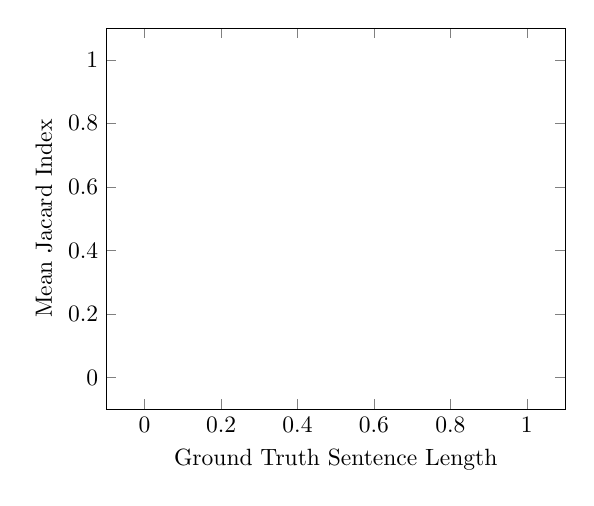
\begin{tikzpicture}[scale=0.85]
	\begin{axis}[xlabel=Ground Truth Sentence Length, ylabel=Mean Jacard Index]
%	\addplot table [y="glove50_jaccard_mean",x="ground_len"]{\sellenscores};
%	\addplot table [y="glove100_jaccard_mean",x="ground_len"]{\sellenscores};
%	\addplot table [y="glove200_jaccard_mean",x="ground_len"]{\sellenscores};
%	\addplot table [y="glove300_jaccard_mean",x="ground_len"]{\sellenscores};
	\legend{50d GLoVE, 100d GLoVE,200d GLoVE,300d GLoVE}					
	\end{axis}
	\end{tikzpicture}
	\hfill
	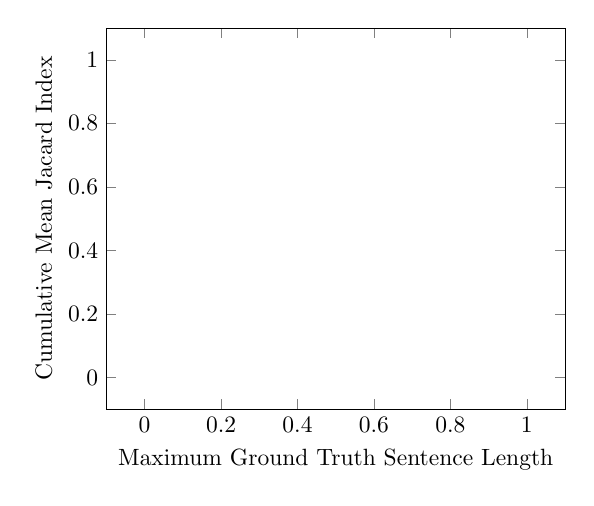
\begin{tikzpicture}[scale=0.85]
	\begin{axis}[xlabel=Maximum Ground Truth Sentence Length, ylabel=Cumulative Mean Jacard Index]
%	\addplot table [y="glove50_jaccard",x="max_ground_len"]{\sellenscorescum};
%	\addplot table [y="glove100_jaccard",x="max_ground_len"]{\sellenscorescum};
%	\addplot table [y="glove200_jaccard",x="max_ground_len"]{\sellenscorescum};
%	\addplot table [y="glove300_jaccard",x="max_ground_len"]{\sellenscorescum};
	%\legend{50d GLoVE, 100d GLoVE,200d GLoVE,300d GLoVE}					
	\end{axis}
	\end{tikzpicture}
	
	\caption{The mean Jaccard index achieved during the word selection step, shown against the ground truth length of the sentence. On the left is the score at each length, and the right is the cumulative score averaged across sentences of up to the indicated length.  Note that the results become noisy for longer sentences, as there are very few long sentences being averaged over -- 75\% of all sentences in the corpus are of length 25 or less. \pdfcomment{LW: Shall I just show a histogram here? RT: Depends on what you want to show. If the sentence distribution is important then you should, but you have indirectly provided this from the current information (in the caption and text) so perhaps not necessary.}}
	\label{figure:exactlenscore}
\end{figure}
\begin{table*}[t!]
	\centering
	\pgfplotstabletypeset[col sep=comma,ignore chars={"},fixed zerofill, precision=3,column type=C{4em},
	columns/Giveups/.style={precision=1, percent style},
	columns/Exact Ordered Matches/.style={precision=1, percent style},
	columns/Exact Ordered Matches Excluding Giveups/.style={precision=1, percent style},
	]{data/ordering_scores.csv}
	\caption{ The overall round-trip performance, including the ordering step with various embedding dimensionalities. Only evaluated on sentences of ground truth length 18 or less. A Giveup occurs when the beam search could not find an ordering with nonzero probability, and so no attempt was made to order the words beyond the order they were found in the selection step. The right hand columns exclude these Giveup cases where ordering failed -- they show only the accuracy when the ordering step suggested it produced a valid ordering at all; the left hand columns are more significant as to the overall performance of the method. The Oracle BOW bypasses the selection step, by providing to the ordering step randomly shuffled reference sentences. It is presented for comparison of the best possible performance using the ordering method.}
	\label{table:ordering}
\end{table*}

\begin{table*}[t!]
	\centering
	INSERT TABLE OF EXAMPLES HERE
	
	\caption{Examples of  }
	\label{table:examples}
\end{table*}


The overall results for the selection step are presented in \Cref{table:overall}. The results plotted against the ground truth sentence length are shown in \Cref{figure:exactlenscore}. It can be noted that the performance improves the higher the embedding dimensionality, and degrades as the sentence length becomes longer. With high dimensional representations it continues to perform well for sentences of reasonable length.


The method is shown to be able to often exactly reproduce sentences based on their embeddings.  Due to its exact and near exact resynthesis of whole sentences it is possible to assess it on a whole corpus, rather than having to demonstrate it only on a few examples. For comparison, results on the examples from \textcite{Bowman2015SmoothGeneration,iyyer2014generating} are shown in \Cref{table:examples}.
It can be noted that  our process does not often generate paraphrases, but rather the original sentence. This is due, at least in part, to the method being able to successful minimise the distance to the original down to zero. Thus resulting in the original bag of words -- rather than a similar sentence.


However the rigidity which allows for the exact reproduction is also seems likely to also cause a limitation, where failures are likely to be ungrammatical e.g. missing conjunctions -- which would cause finding a reasonable ordering to be impossible -- without further processing to repair. This would cause the any search of the ordering graph to return no results.


The results on the overall process are shown in \Cref{table:ordering}. These results show the performance of ordering the output of the previous selection step, at the various different embedding dimensionality. Shown also is a Oracle BOW, where the selection step is bypassed, to establish an upper bound on the performance. For the Oracle result, the bag of words input comes just from shuffling the words in the reference sentence.

The high score of the Oracle BOW, confirms the hypothesis that for most sentences the word order can be inferred from the word content alone -- but certainly not all. This presents an upper bound on the performance of any method attempting to regenerate sentences from embeddings which do not preserve word order. 

It can be that a very significant portion of the failures come from the ordering step ``Giving up''. A give-up occurs if the beam search failed to find any ordering to which non-zero probability was assigned. This could be because the ordering was outside of the search width, or because no reasonable ordering was possible. The former can be solved with a wider beam search -- or switching to a complete search in general. The later can only be solved by making less errors in the word selection step. Both issues certainly occur. 

When the sentences which are given-up on are excluded, the ordering performance actually gets worse as the dimensionality increases. This is because the lower dimensional models output invalid word combinations in the selection step for more difficult sentences -- those which are more likely to be ordered incorrectly even if the selection is done perfectly.




\section{Conclusion} \label{conclusion}
A method was presented for how to regenerate a bag of words, from the sum of a sentence's word embeddings. The word selection problem, of going from the sum of embeddings to the words, is NP-Hard. A greedy algorithm was found to perform well at the task, particularly for shorter sentences when high dimensional embeddings are used. It was also demonstrated that a simple probabilistic language model can be used to order the bag of words output to regenerate the original sentences.

Resynthesis degraded as sentence length increased, but remained strong with higher dimensional models up to reasonable length. The fairly basic beam-search based ordering technique was only evaluated on sentences with up to 18 words (inclusive), due to computational time limitations. On these it performed quite well with the best model achieving perfect recreation 80.7\% of cases. Performances, both accuracy and running time, is expected to worsen were longer sentences considered. With that said, 18 words is sufficient for many uses.

From a theoretical basis the resolvability of the selection problem shows that adding up the word vectors does preserve the information on which words were used; particularly for higher dimensional embeddings. This shows clearly that collisions do not occur (at least with frequency) such that two unrelated sentences do not end up with the same SOWE representation. 

\subsubsection{Future Work}\label{future}
One of the restrictions placed during the evaluation of the technique was that pretrained embeddings must be available for all words, which is reasonable as the embeddings can always be trained to include those words. Another technique we have been developing is to assign missing words a vector of zero. This results in them never appearing in the generated BOWs. However assuming they do appear in the language model training corpus, they can be inserted during the ordering step. If it is more likely to have that missing word, than to not. This technique showed promising results when used with the \texttt{word2vec} vectors \parencite{mikolovSkip}, which exclude common stop words like ``to''. This technique also has the potential to allow for mistakes made in the selection step, for example do to noise in the process outputting the vectors, to be corrected in during the ordering step.




\printbibliography
	
\end{document}


